\chapter{Implementation}
\label{chapter:implementation}

%You have now explained how you are going to tackle your problem. 
%Go do that now! Come back when the problem is solved!

%Now, how did you solve the problem? 
%Explain how you implemented your solution, be it a software component, a
%custom-made FPGA, a fried jelly bean, or whatever.
%Describe the problems you encountered with your implementation
%work. Sometimes the content of the environment chapter is combined
%together with the implementation chapter.

In this chapter we will introduce the software created for this thesis and the challenges faced while developing it.
This chapter is divided into two parts.
In the first part we will examine technically what was the end result while quickly commenting on some of the choices that can be seen in the final architecture.
Because of time constraints and challenges during development, there were some parts such as HBase as a storage which we could not develop.
These challenges are explained in the latter part of this chapter and we continue with them in the following evaluation chapter.

\section{Overview}

In this section we will explain the practical application that was developed.
We start by addressing some of the deadends that lead to the final pipeline to give reader a clearer view what changed in practice after the previous chapter.
Some of the reasoning why some of the technologies were prioritized leading to not being to test every technology is presented here but more in-depth look at for specific integrations and problems will be examined in the next section.
Finally in the section 5.1.3, we introduce how the pipeline can be run with any novice data scientists local machine.

\subsection{Dead-ends at the start of development}

Two technologies that were mentioned in the previous chapter were eliminated at the start of the development of each.
These were Apache Flume and Apache Cassandra.
As both seemed to lead to a dead-end in the development and there existed seemingly better alternatives than these, focus was moved to other technologies.

Apache Flume was supposed to be used as a component in the ingestion step, but due to its charasteristic of being mostly aimed at data which could be fetched in log form, it could not be used with the REST APIs that most of the data services use.
Flume also did not seem to have any native ways to connect to storages such as Cassandra.
There exists some ready-made solutions for this, but these were unmantained and seemed possible dead-ends.
This is why Flume was ruled out.

Apache Cassandra was dropped from the development mostly because integrating it with other services would have required a lot of extra work. 
Further examination of Cassandra also showed that Cassandra is not very good choice for this specific purpose that we want to use it for.
Cassandra is known for its ability to write enormous volumes of data, but when it is time to read from the storage the task becomes non-trivial.
Reading from Cassandra is based on the Cassandras query language, CQL, which allows somewhat efficient queries but you have to define these high perfomance queries at the time you create tables for data. \cite{dronavalli}
Because our pipeline should be used mostly by analysist who can have varying queries into the storage this raises a challenge for future development.
This is why we decided to discontinue with Casssandra.

\subsection{Final Architecture}

% for screenshots
\begin{figure}[ht!]
    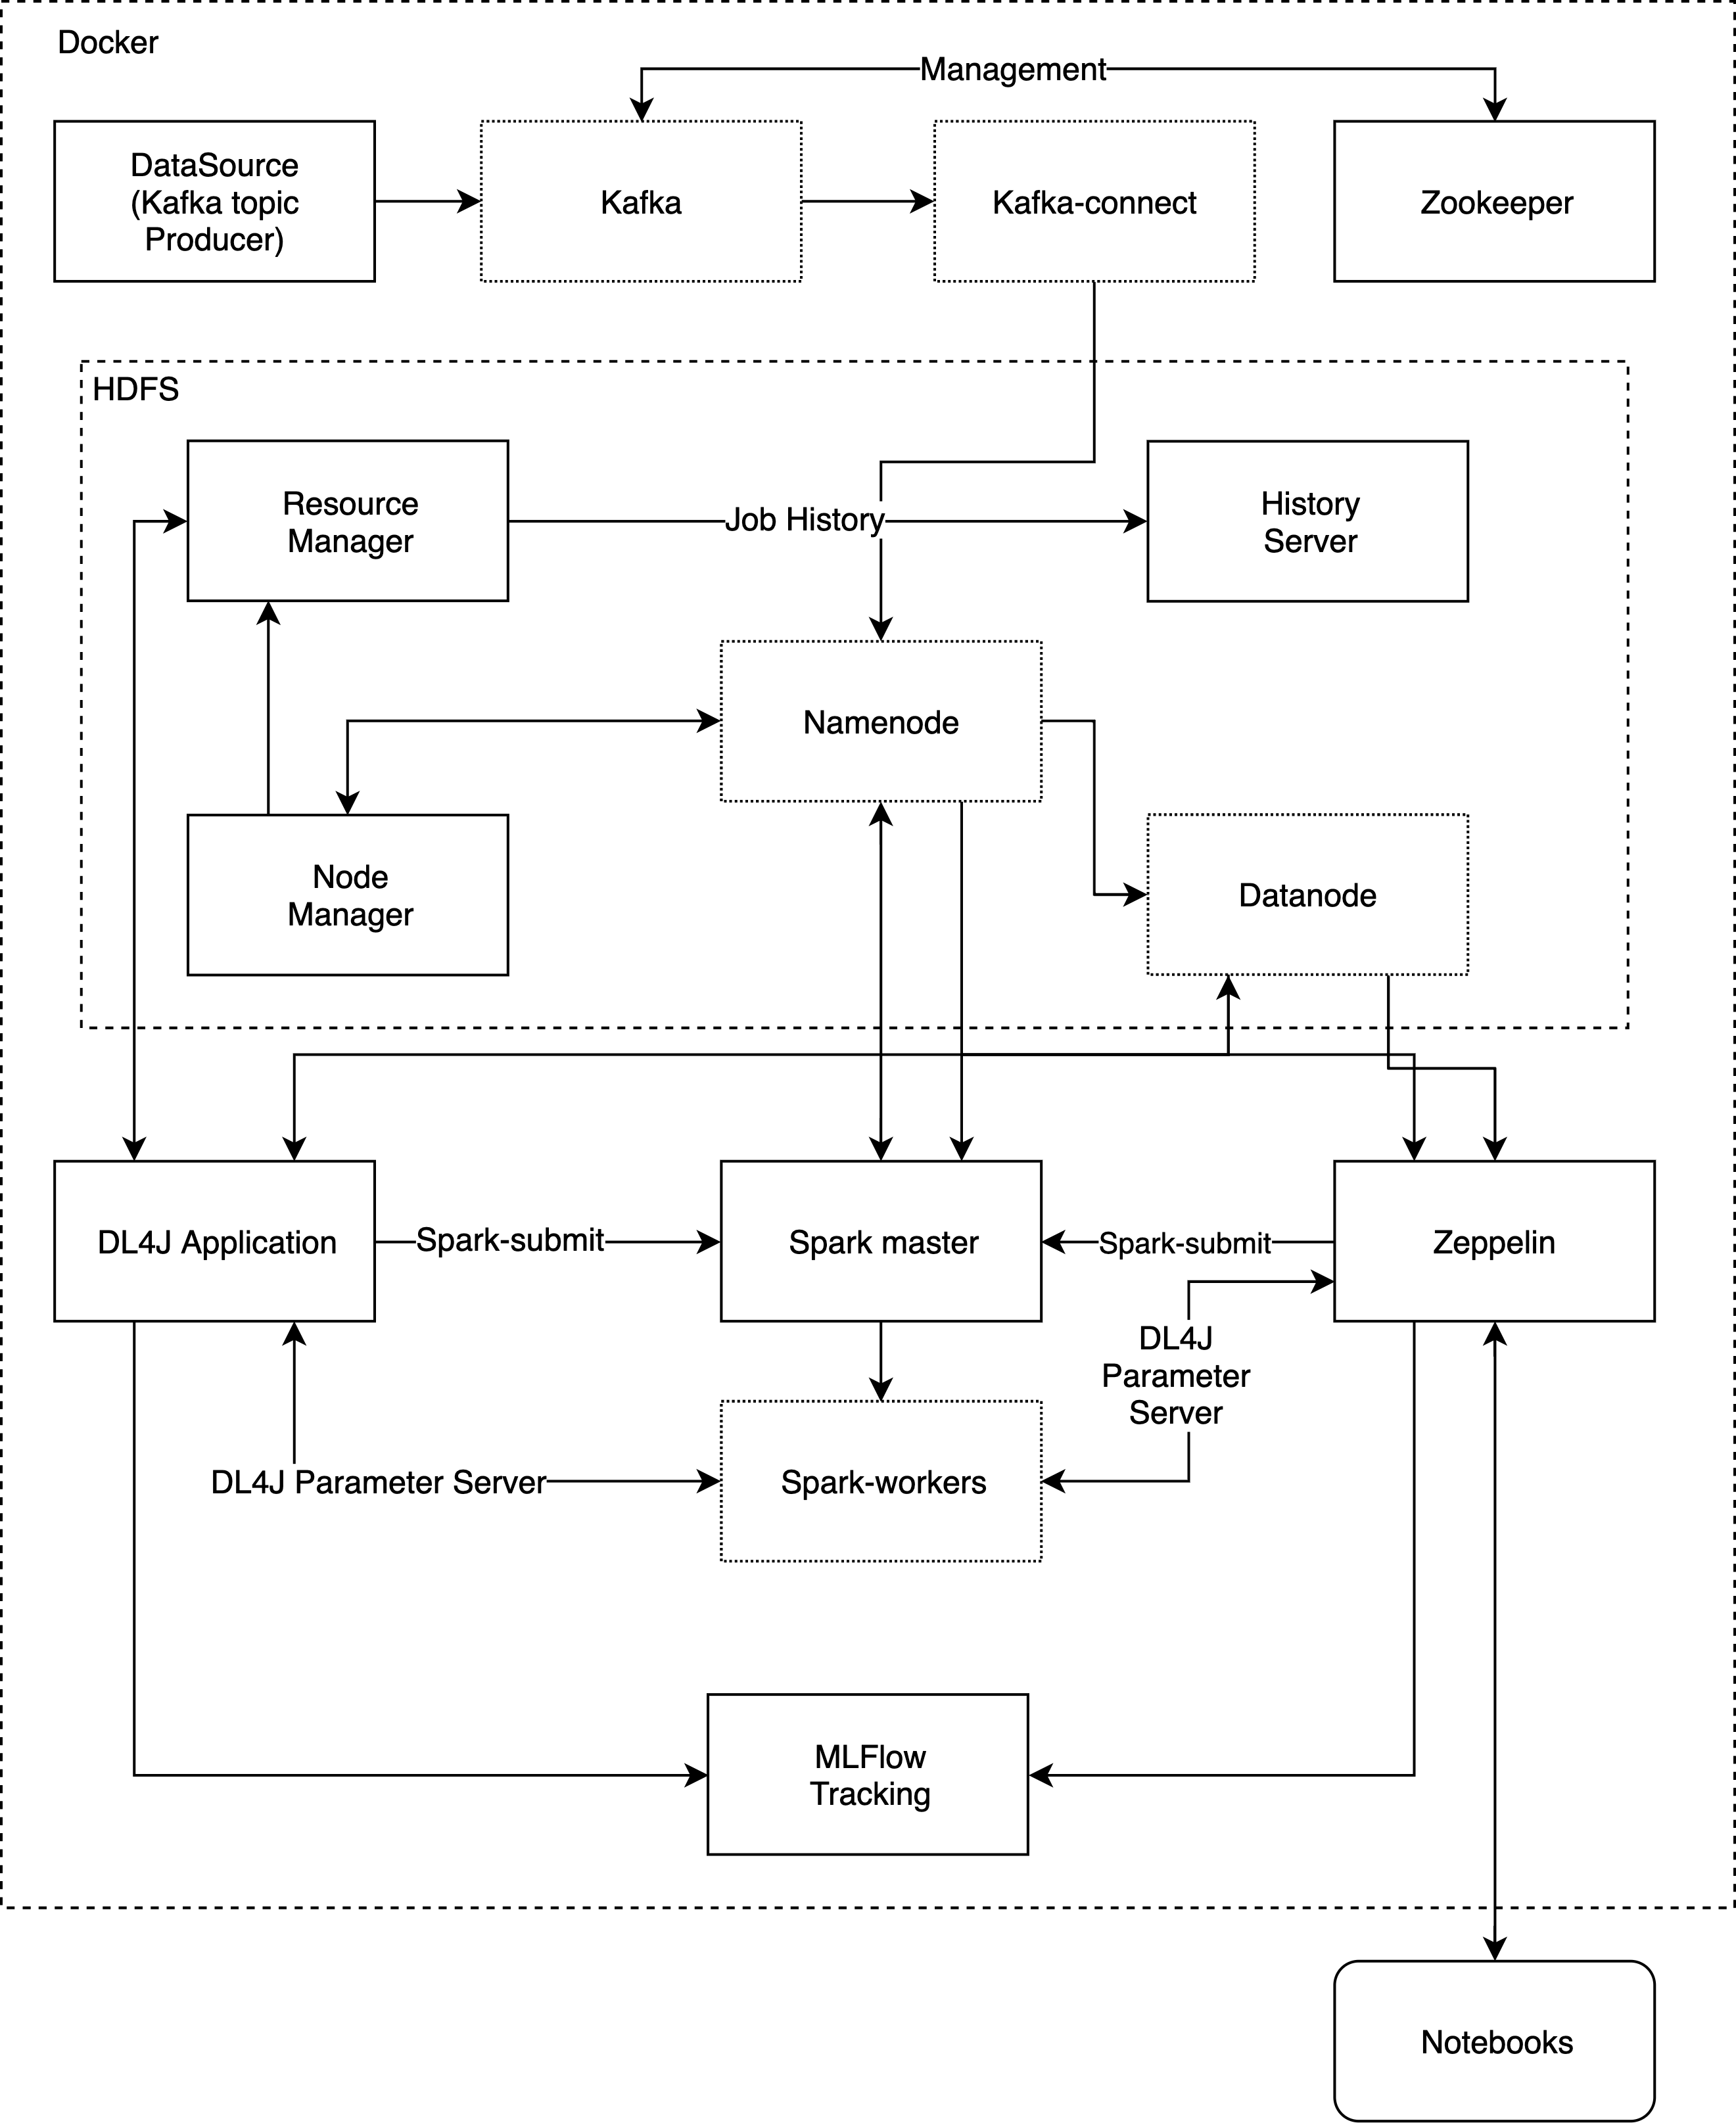
\includegraphics[scale=0.20]{images/architecture} 
    \centering
    \caption{Final Architecture of the implementation section}
\end{figure}

The final architecture can be seen in the figure 5.1.
The figure presents the main dependencies between the components each arrow usually presenting the flow of data in the system with labels sometimes added to clarify better the relation.
In the figure each solid rectange represents one actual server with its own process with the exception of rounded rectange to represent notebooks that are stored into the local file system.
In the case of this thesis these servers were virtual machines but theoretically the system could be run with right configuration with multiple physical machines that are in the same network.
Rectangles with small dashed lines such as with the spark workers represent that the server can have easily more than one instance allowing horizontal scaling.
The longer dashed lines here represent bigger entities such as the HDFS cluster to make the figure more readable.

The pipeline starts from the data source that acts as the kafka producer.
It reads the data from a source, in this example case from JSON files, and produces the data into a kafka topic. 
It also creates the needed kafka topics on startup using Kafkas admin API.
Although most of the kafka documentation recommends using the command line client, this did not seem production-ready way to do this as this decouples the topic creation logic from the actual producer and would need excessive scripting in order to automate this process which did not seem as maintainable as the admin API approach.
This is why admin API was used in the data source server. 

Then we have Kafka which is integrated into HDFS cluster with Kafka Connect HDFS 2 Sink connector which is a component made by Confluent.
This acts as a kafka consumer and listens to the topic that the producer defines.
Connect can be scaled and contains some basic configurations that can be used for example to define the format in which the data is stored into HDFS.
We have chosen JSON as the format which the data is stored but Apache Avro is also an option.
Other notable configurations that can be used to tweak the pipeline are the rate in which the topic is consumed into the HDFS and schema validation.

In the middle of the pipelin is the HDFS cluster.
In this cluster there is the normal HDFS cluster with namenodes and datanodes which can be accessed to directly read the data.
There is also a YARN resource management on top of this which can be used to for better manage IO routines in the cluster.
This consist of the resource manager, node manager and history server nodes, that can be used as an alternative route to access data.

The HDFS cluster docker containers, as well as the containers for Spark cluster later, are a work of Big Data Europe project.
The Big Data Europe is project funded by European union which one of the goals is to produce open-source tools for big data development without the need to use closed softwares.\cite{bigdataeurope}
As these containers were the most maintained hadoop containers at the moment of writing this, they are were the best option for this case, but they brought a couple of problems which we will examine later.

\begin{table}[! htbp]\centering
    \caption{Storage and ingestion components versions}
    \begin{threeparttable}
        \begin{tabular}{|c|c|c|c|c|c|c|} 
        \hline
        & Hadoop & Kafka & Kafka Connect & Zookeeper \\ \hline
        Version & 3.1.1 & 2.3.0 & 5.2.1 & 3.5.5\\
        \hline
        \end{tabular}
    \end{threeparttable}
\end{table}

In table 5.1 we have gathered the versions of the technologies used in the first half of the pipeline.
Most are the newest versions of each software at the writing of this.
The version of hadoop is specially tricky as its clients are used in multiple parts of the pipeline coupled with other software libraries which have support for only some of the older versions but do not complain if used with the newer one.
This is why there can be other versions than this in the pipeline e.g in the spark cluster, but as they do not currently cause any visible errors and due to the time constraints that this project has, the versions can mismatch for now.

After the HDFS cluster comes the analysis part of the pipeline which has Spark cluster in the middle and two options to run analysis code on it.
The application part allows writing production grade scala applications that can be run like any normal scala spark application.
The Zeppelin is a Apache Zeppelin instance which allows writing and running notebooks that can be saved into local file system for distribution.
Both approaches submit the spark application to spark using spark-submit script and the DL4J communicates with itself with its own parameter server.

In default case, the spark application first preprocesses the json formatted data and saves this back to HDFS as csv files.
In this process, it normalizes the data and appends labels to it that in our example case is just values 1 and 0 whetever the value of stock grew in n-days after the datapoint or not respectively.
The data is stored back as a CSV file because DL4J is quite picky about the data format that it accepts and does not have simple default way of transforming spark DataFrames with sequential data to the Dataset format that it internally uses.
After this the data goes through the training and evaluation pipeline which logs its parameters and results into MLFlow server where user can monitor the process of their different experiments.

\begin{table}[! htbp]\centering
    \caption{Analysis Software versions}
    \begin{threeparttable}
        \begin{tabular}{|c|c|c|c|c|c|c|c|} 
        \hline
        & Spark & Scala & Java & DL4J & sbt & Zeppelin & MLFlow \\ \hline
        Version & 2.4.3 & 8.x & 2.11.12 & 1.0.0-beta5 & 1.26 & 0.8.1 & 1.2.0\\
        \hline
        \end{tabular}
    \end{threeparttable}
\end{table}

In the table 5.2 we have collected the versions of different components in this part of pipeline.
Almost all of them are the latest releases of each technology at the time of implementing with the exception which is the version of Scala.
Currently, the latest version of Scala is 2.13.
Spark mainly supports scala 2.12, because as of 2.4.1 version of spark, the version 2.11 of scala is deprecated and there is still no support for 2.13.
However, Zeppelin does not support Scala version 2.12 so the only version of Scala that still works with all of the latest releases of these two technologies is 2.11 which is why it had to be chose for the version.
Java is still version 8 which is already at its end of life stage, but it was used as it is currently the safest way to ensure that your code runs correctly.

\subsection{Usage}

The initial idea of the project was to provide modular design for the pipeline where the user can cut and paste the technologies to the pipeline making it easy to produce multiple different pipelines for comparison.
That is why the there is a initialization script called pipeline.sh.
This is a command-line interface that asks user what technologies they want and builds a docker-compose file into build folder with all the necessary files.
Sample usage is depicted in the figure 4.2.
Only thing user has to do before running the script is to download manually the Kafka Connect component from confluent website and copy its content to a location noted in the project readme. 
This step is mandatory because unfortunately Kafka Connect did not have public distribution that would have allowed access without authentication.
If this component is missing during the build, the initialization script notifies user about this before continuing further.

After the initialization, using the software is the same as with any other normal docker-compose project.
Users can copy the contents of the build folder as the base of their own project or use it as it is.
The project can then be build with "docker-compose build" command and run using the command "docker-compose up".
After this as there will be over 10 containers running simultaneously, tools such as lazydocker are recommended for proper management.

When the containers have finally finished the startup procedures, every services user interface can be found in their default ports in localhost.
The ports needed to be open to this happen, can be found in the docker-compose.yml file.
To start analysing data, the user has to only open localhost:8090 where Zeppelin notebooks are running.
In the project there exists an example notebook that implements a simple LSTM model.
To run this example on spark cluster user has to first manually set two configurations in the spark interpreter menu that can be found under interpreter settings in the user interface.
The value "master" must be set to "spark://spark-master:7077" in order to let the zeppelin use the cluster instead of local spark client.
Also in the dependencies has to be added "org.apache.commons:commons-lang3:3.6" in order to have common versions in the zeppelin machine and in the cluster.
The reason for the manuality of these tasks will be discussed in following sections.
After this the user has to only run the cells in the notebook and the result will be saved into HDFS.

To add third party dependencies to the notebooks such as the DL4J library, the "spark.deb" syntax in notebooks is encouraged as this is the best way to preserve the dependencies for possible distribution of the notebook.
This way the notebook is as independent of its environment as it can be.
It is currently also the only way to preserve these if the container happens to be destroyed. 
Reasons for this will again be discussed in following sections.

\section{Adversities during development}

Most of the time during development went to trying to integrate these services with each other.
The reason for this was mostly features that were not documented well and other misshaps such as bugs that happen when integrating two services that are not that common together.
There was a lot of unique problems that did not have any documented solutions on the internet which made solving them very time consuming.
In this section we will be going through the ones that took most time to solve and present the solutions at high level to these problems.
More precise technical problems with their solutions can be found in this thesis' git repository that contains all the practical results.

\subsection{Kafka-HDFS integration}

Integrating Kafka topics to HDFS proved to be a non-trivial task.
Unlike products like Flume, Kafka does not have any build-in sinks that would allow easy integration of different services.
So the developer is left with the task of filling this hole.

The requirements for this component are also non-trivial, as it should be able to scale with the kafka and the HDFS cluster.
So in order to not introduce a bottleneck to the pipeline and to do this with time limits that this thesis has, a ready-made solution was necessary.
Previously, a good solution to this has been Linkedin's Camus API, but this was phased to Apache Gobblin in 2015. 
The problem with Apache Gobblin, however, is that it is not the lightest tool and it can move data only to Hadoop system.
That is why if we were to change the HDFS storage to try some other storage option, the Gobblin should be entirely changed to something else.

Technology that solves these problems is Kafka Connect. 
Kafka Connect acts like a sink plugin to Kafka.
Unlike with Gobblin, developers can download only the sink they actually need instead of sinks for every possible case.
Because Kafka Connect has sinks for most major big data storages in the market, user is not constrained as much to Hadoop ecosystem like with the Gobblin.

The downside is that Kafka Connect is clearly Confluent product although it is open-sourced and free.
Confluent has its own platform that it promotes as open-source event-streaming platform that can be used as a enterprice solution. 
This is why most of the Kafka Connect documentation is only about how to use it on top of this Confluent platform, although it has capabilities to run independently.
This lack of good documentation introduced some obstacles for integrating this component between Kafka and HDFS especially when it came to installing and running the component.

Setting up the Kafka Connect was not that easy as it does not offer much monitoring in itself.
This means that as developer you could only see if the whole system worked or did not from HDFS management console.
If only some configuration was not right, Connect would only log this as an minor error in the stderr and continue running like nothing had happened although no data was flowing through it.
This made debugging the connection surprisingly difficult, but after all the configurations were in place the component worked as it should throughout the rest of the development.

\subsection{Apache Zeppelin dependency management}

Major problems came when the development reached to the point of adding DL4J dependencies to the Zeppelin instance.
Zeppelin has multiple ways of adding dependencies and the main way that is defined in its documentation is by its dependency UI that is located in its interpreter settings panel.
This again saves these settings into interpreter.json file which is a normal JSON configuration file.

At the start of this development in order to remove the manual step of adding dependencies and other settings, we tried to save this interpreter configuration file between container restarts.
This worked with every other setting except dependencies.
Dependencies would conflict for unknown reasons and and the error message would change per restart.
Sometimes by mere luck the dependencies would build correctly for a certain amount of time but then fail again.
This would be easy to debug if Zeppelin would be a normal maven project as it is.
But with ready-made containers there did not exist such an option.

Apache Zeppelin has official container which were used, but this had to be extended in order to have custom spark-submit client because the versions on spark cluster would conflict.
When thought afterwards, the whole zeppelin container probably should have been build from scratch as this would have allowed better dependency management with maven.

\subsection{DL4J sbt project}

The DL4J application instance without Zeppelin is build with sbt.
sbt is a build tool developed specifically for Scala applications and this why it was also chosen for this project.
DL4J's main build tool that the documentation is build around is maven because it is a Java library, but it has its own sbt example in their project repository.
This, however, turned out to be highly outdated and caused developing problems.

To have third-party dependencies added to a spark project there are two possible ways to implement this.
First one is using the spark-submit scripts flags to define maven repositories.
This was first tried but it only lead to dependency conflicts and other bugs with ivy dependency management that the script uses.

The alternative and more manageable way is to build the whole application into so called fat jar, which contains all the code to run the application including the third-party dependencies.
This is what the outdated sbt example did so we opted to update this example to work with newer versions of sbt and sbt-assembly which is a plugin needed for building fat jars on sbt.
To make the example project work, we migrated it from sbt version 0.X to sbt version 1.X syntax. 
The migration of general syntax was relatively easy, but with the newer version of DL4J library, a new merge strategy had to be written for sbt-assembly.
Merge strategy is what sbt-assembly uses when it encounters duplicate files during the building process.
Writing a updated merge strategy for DL4J was not a trivial task as the strategy that was usually suggested did not work in this case and lead to errors in runtime.
After quite a bit of trial and error, we thankfully managed to create a merge strategy that did not throw away necessary files needed at the runtime.

\subsection{Running the application in Spark}

Now we move on to the problems that were really hard to debug when the problems in the previous two subsections were persisting at the same time.
When running a Zeppelin task on Spark and the program receives error, Zeppelin correctly logs the stack trace from Spark workers stderr.
What it does not do, is logging the the whole stack trace but only the two to three first errors.
This made it seem like the error was a some upper level error when instead the actual error that happened in lower part of the stack.
This was resolved by noticing the full stack when the application was run on application server.

After this, the next problem was that Intels mkl-dnn library did not seem to be in the classpath of DL4J subdependency library javacpp.
This is the code that is responsible of allowing the java code to use high efficiency feature of C++ language.
This of course did not have any clear solutions online except some vague conversation logs about possibility of glibc missing in the parent OS and by accident this turned out to be the exact problem in this case too.
The Spark worker docker container, which was a result of the Big Data Europe project, was build on top of alpine linux image which has phased out to use musl libc library instead of glibc.
There exists tools that can be used to install glibc to alpine instance and we tried this, but after multiple errors in multiple different attempts to install the library, we opted out to fork the docker image to use debian based image.
This resolved all the problems that had been until this point and the application finally compiled in worker machine.

The problems after this did not cause the application process on worker to crash but were logged into worker machine while the process continued to run.
These were somewhat minor but laborous problems such as allocating enough disk for /dev/smh shared memory implementation and opening and defining right ports for DL4Js parameter server that handled the parameter update logic.
Once all of these were fixed, the next problem was that the training process in spark did not finish at all and seemed to go into a state of infinite loop without giving any errors on the driver logs.
This seemed like a dead-end until we noticed that a spark job before this had silently failed.
It seems that the DL4Js training code was beforehand trying to temporarily save the data into hdfs and this failed as something went wrong.
This step in the process could be skipped with configurations and after this the model training process finally succeeded.

The final problem we faced was a randomized index out bounds exception.
Raising the number of epochs we noticed that this occured at random, and unlike the previous errors, this seemed like a error in the library.
The code that raises this error handles parallel code so if we were to make conjectures from this it would seem like there would be an error with shared memory access in some part of the asynchronous code.
However at this point, the time allocated to this project was already running out so we could not confirm this definitely.

Now that we have seen what we were able to implement during this thesis we move on to evaluate the quality of this software.
We will also discuss more about what went well, what went wrong and what could have been done better.